\section{Taxonomy: Five Evolution Loops}
\label{sec:taxonomy-five-loops}

AI self-evolution is best understood not as a single algorithm, model family, or benchmark, but as a family of feedback loops that repeatedly transform a system from one operational state into another.  The shared pattern is simple: a system proposes variants, evaluates them, keeps some information about what happened, and uses that information to change its future behavior.  What differs across the literature is the object being changed, the source of feedback, the persistence of the update, and the scale at which alternatives are maintained.  A self-refining answer changes a text output over several inference-time iterations; a reflective agent changes its memory; an AutoML agent changes an executable pipeline; a program-evolution system changes source code; a population method changes an archive of candidate agents or algorithms; and a training-time self-play method changes model parameters.  The common abstraction is an evolution loop, while the practical field is organized by the kinds of loops that are composed.

This chapter proposes a taxonomy around five recurring loops: the specification-to-execution loop, the search loop, the evaluator loop, the reflection loop, and the population loop.  These loops are not mutually exclusive.  They are modular mechanisms that can be layered.  For example, a system such as AlphaEvolve can be read as the composition of search, evaluator, and population loops; ADAS can be read as specification-to-execution plus search over agent designs; Reflexion combines evaluator signals with reflection memory; FunSearch couples candidate program generation with executable evaluators and evolutionary selection; and AutoML-Agent turns natural-language objectives into a multi-agent pipeline whose outputs can be evaluated and revised.  The taxonomy is therefore not a set of boxes into which each method must fit exactly.  It is a vocabulary for decomposing systems, comparing them, and designing future self-evolving AI infrastructure.

The central distinction is between \emph{where} the update happens and \emph{what} feedback makes it legitimate.  A prompt-level method updates a message, rationale, or instruction.  A memory-level method stores natural-language lessons or trajectories.  A pipeline-level method modifies a workflow, tool choice, feature transform, or agent role.  A code-level method edits a program or agent implementation.  A population-level method changes an archive of variants.  A weight-level method performs training or reinforcement learning.  Evaluation can likewise range from soft self-critique to human preference, unit tests, benchmark scores, code execution, deployment metrics, or formal validators.  The more persistent and consequential the update, the stronger the evaluator normally needs to be.  A one-step wording revision can tolerate a weak critic; a system that changes source code, agent permissions, or model weights requires regression tests, sandboxing, rollback, and audit trails.

The five-loop view is useful for survey work because it connects several research traditions that often use different terminology.  AutoML emphasizes task specification, pipeline construction, and metric-driven optimization.  Neural architecture search emphasizes candidate generation, search spaces, and performance estimation.  Evolutionary computation emphasizes populations, mutation, crossover, diversity preservation, and selection.  Program synthesis emphasizes executable candidates and test-based repair.  Agent research emphasizes planning, tool use, memory, multi-agent coordination, and reflection.  LLM self-improvement emphasizes iterative feedback, synthetic data, self-play, and model updates.  Self-evolution emerges when these traditions are combined into a system that can repeatedly improve its own artifacts or behavior under evaluation.

\subsection{Unified Formalization}
\label{subsec:taxonomy-formalization}

Let $z_t$ denote the state of a self-evolving AI system at iteration $t$.  The state may include a model, prompt, memory, agent workflow, source-code repository, benchmark log, archive of candidates, data buffer, or any combination of these artifacts.  A candidate-generation operator $g$ maps the current state to one or more proposed variants.  An evaluator $e$ maps candidates, execution traces, or artifacts to feedback.  A selection operator $s$ chooses which candidates or feedback items matter.  An update operator $u$ incorporates the selected information into the next state.  A compact evolution equation is
\begin{equation}
  z_{t+1} = u\bigl(z_t, g(z_t), e(g(z_t))\bigr),
  \label{eq:general-evolution-loop}
\end{equation}
where $g(z_t)$ may be a single candidate or a set of candidates.  When explicit selection is useful, the same loop can be written as
\begin{equation}
  C_t = g(z_t), \qquad F_t = e(C_t; z_t), \qquad A_t = s(C_t, F_t, z_t), \qquad z_{t+1}=u(z_t,A_t,F_t).
  \label{eq:expanded-evolution-loop}
\end{equation}
Here $C_t$ is a candidate set, $F_t$ is a feedback object, and $A_t$ is the accepted subset or action chosen by selection.  The feedback object may contain scalar scores, pass/fail tests, natural-language critiques, symbolic gradients, execution traces, counterexamples, confidence estimates, cost measurements, or safety violations.  The accepted subset may contain a single best candidate, the top $k$ candidates, a diverse archive, a revised prompt, a new memory entry, or a set of training examples.

The formalization deliberately separates generation from evaluation.  In many LLM systems, the same foundation model participates in both steps: it proposes an answer, critiques it, and revises it.  Nevertheless, the roles are conceptually distinct.  Candidate generation answers the question: \emph{what should we try next?}  Evaluation answers: \emph{how did it perform?}  Selection answers: \emph{what should be trusted or retained?}  Update answers: \emph{what persistent change should be made?}  Keeping these roles separate makes it easier to compare methods with different implementations.  Self-Refine uses an LLM as both generator and critic, but its update is mostly a revised output.  Reflexion uses environment feedback to write natural-language memory, so its update persists across attempts.  FunSearch uses an LLM to generate programs and a programmatic evaluator to score them, so its update is an archive of better programs.  AutoML-GPT uses natural-language task descriptions to generate ML pipeline components, and the evaluation includes training logs and metric estimates.  DGM and AlphaEvolve move the update into code and population archives.

A useful design decomposition is to treat $z_t$ as a product of layers,
\begin{equation}
  z_t = \bigl(m_t, p_t, a_t, c_t, d_t, h_t, \pi_t\bigr),
  \label{eq:state-factorization}
\end{equation}
where $m_t$ denotes model parameters, $p_t$ prompts or instructions, $a_t$ an agent architecture, $c_t$ source code, $d_t$ data or demonstrations, $h_t$ history and memory, and $\pi_t$ policies for evaluation, routing, or selection.  Different self-evolution methods operate on different coordinates of this state.  A reflection loop mostly modifies $h_t$ and sometimes $p_t$.  A prompt optimizer modifies $p_t$.  AutoML and ADAS modify $a_t$, $c_t$, or workflow policies.  Code-evolution systems modify $c_t$.  Self-play and reinforcement-learning systems modify $m_t$ and $d_t$.  Population methods modify a collection of states, $\mathcal{Z}_t = \{z_t^{(1)},\ldots,z_t^{(n)}\}$, rather than a single state.  This factorization also clarifies why safety requirements differ.  A temporary answer revision is reversible; a memory update can bias future behavior; a code update can break a toolchain; a weight update can change the entire capability surface.

The candidate-generation operator $g$ may be implemented in several ways.  It may be a direct LLM sampler conditioned on task instructions and history, as in prompt optimization or code generation.  It may be a planner that decomposes a natural-language goal into subgoals, as in AutoML and agent frameworks.  It may be a mutation operator over program text, graph structures, neural architectures, hyperparameters, or prompts.  It may be a crossover operator that combines multiple candidates.  It may be a learned controller, a reinforcement-learning policy, a Bayesian optimizer, a symbolic transformation rule, or a multi-agent deliberation protocol.  In modern self-evolution systems, the distinctive feature is that $g$ is often semantic: the generator can read comments, tests, traces, and prior failures, and can propose structured changes rather than random edits.

The evaluator $e$ is the central source of legitimacy.  A weak evaluator supplies verbal plausibility, stylistic preference, or self-consistency.  A medium-strength evaluator supplies external feedback such as answer correctness, reward, human preference, or benchmark score.  A strong evaluator supplies executable, repeatable, and automatically checkable evidence: unit tests, formal constraints, compilers, proof checkers, simulators, held-out benchmarks, runtime monitors, or deployment metrics.  The quality of self-evolution is bounded by evaluator quality.  If the evaluator is noisy, the loop may overfit, reward hack, or preserve candidates that look good only under the local test.  If the evaluator is expensive, the loop may become sample inefficient.  If the evaluator omits safety constraints, the loop may improve task metrics while degrading robustness, interpretability, fairness, or cost.

Selection $s$ is sometimes implicit.  Self-Refine accepts the revised answer after a fixed number of iterations.  Reflexion records a reflection after failure and conditions the next trial on memory.  OPRO-style optimization ranks candidates by scalar score and asks an LLM to propose better ones.  Population methods make selection explicit: they keep elites, replace dominated candidates, maintain niches, or sample parents according to fitness and diversity.  Selection can be single-objective, multi-objective, risk-constrained, novelty-seeking, or human-gated.  It can be greedy, tournament-based, Pareto-based, archive-based, or curriculum-based.  In self-evolving agents, selection should normally account not only for reward but also for stability: a candidate that improves one benchmark while breaking another should not automatically replace the incumbent.

The update $u$ is what distinguishes mere iterative inference from self-evolution.  If no persistent state changes, the loop is an inference-time refinement pattern.  If a memory is updated, the system evolves across attempts.  If prompts, tools, code, or weights are changed, the system evolves across deployments.  The update can be soft, such as appending a reflection to memory; structural, such as adding an agent role; executable, such as editing a function; statistical, such as fine-tuning; or organizational, such as changing which specialist agents are invoked.  In practice, a robust update function includes rollback, provenance, confidence thresholds, and regression checks.  The update should answer: what changed, why it changed, what evidence supports it, and how it can be undone.

The following diagram summarizes the common loop.  It is intentionally abstract: each box can be instantiated by a prompt, model, agent team, compiler, benchmark harness, training job, or archive manager.

\begin{figure}[t]
\centering
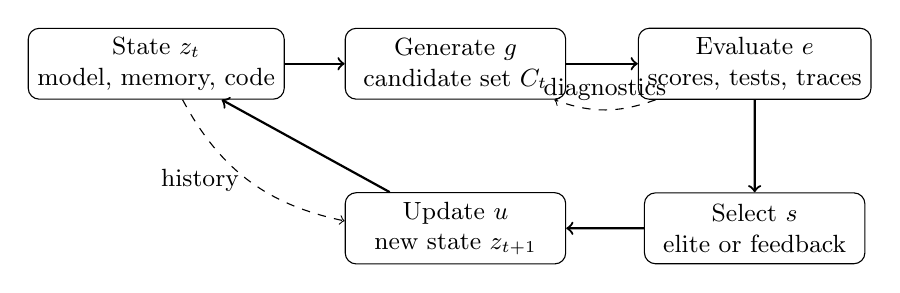
\begin{tikzpicture}[scale=0.95, every node/.style={font=\small}]
  \node[draw, rectangle, rounded corners, align=center, minimum width=2.8cm, minimum height=0.9cm] (state) at (0,0) {State $z_t$\\model, memory, code};
  \node[draw, rectangle, rounded corners, align=center, minimum width=2.8cm, minimum height=0.9cm] (gen) at (4,0) {Generate $g$\\candidate set $C_t$};
  \node[draw, rectangle, rounded corners, align=center, minimum width=2.8cm, minimum height=0.9cm] (eval) at (8,0) {Evaluate $e$\\scores, tests, traces};
  \node[draw, rectangle, rounded corners, align=center, minimum width=2.8cm, minimum height=0.9cm] (sel) at (8,-2.2) {Select $s$\\elite or feedback};
  \node[draw, rectangle, rounded corners, align=center, minimum width=2.8cm, minimum height=0.9cm] (upd) at (4,-2.2) {Update $u$\\new state $z_{t+1}$};
  \draw[->, thick] (state) -- (gen);
  \draw[->, thick] (gen) -- (eval);
  \draw[->, thick] (eval) -- (sel);
  \draw[->, thick] (sel) -- (upd);
  \draw[->, thick] (upd) -- (state);
  \draw[->, dashed] (eval) to[bend left=20] node[above]{diagnostics} (gen);
  \draw[->, dashed] (state) to[bend right=25] node[left]{history} (upd);
\end{tikzpicture}
\caption{A general self-evolution loop.  Candidate generation, evaluation, selection, and update may be implemented by LLM prompting, agent workflows, benchmark harnesses, code execution, population archives, or model training.}
\label{fig:general-evolution-loop}
\end{figure}

The five loops described in the rest of the chapter are specializations of this abstraction.  The specification-to-execution loop emphasizes how a human goal becomes an executable artifact.  The search loop emphasizes how alternatives are explored.  The evaluator loop emphasizes how fitness is measured and guarded.  The reflection loop emphasizes how failures become reusable knowledge.  The population loop emphasizes how many candidates are maintained, diversified, and recombined.  These loops are orthogonal enough to be analyzed separately, yet they become powerful when composed.

\subsection{Specification-to-Execution Loop}
\label{subsec:taxonomy-spec-to-exec}

The specification-to-execution loop converts a natural-language goal into an executable machine-learning or agent pipeline.  It is the loop closest to the product experience of self-evolving AI: a user describes what they want, and the system builds a working artifact that can be trained, evaluated, deployed, or revised.  The input is usually under-specified.  A request such as ``build a classifier for customer churn,'' ``design an agent for web research,'' or ``improve this repository on a benchmark'' does not fully specify data schemas, preprocessing, model classes, hyperparameters, evaluation protocols, runtime constraints, or failure handling.  The loop therefore begins by expanding the user goal into a structured task representation.

AutoML-GPT is representative because it uses an LLM as a bridge between human-readable descriptions and AutoML components.  The system can reason over task cards, model cards, data cards, and training logs, then produce choices for preprocessing, model architecture, hyperparameter optimization, or log prediction.  Its importance for self-evolution is not merely that it automates AutoML.  It shows that natural language can serve as a high-level genome for ML experimentation.  The user's description does not directly execute; it is compiled into a pipeline.  Once the pipeline runs, its metrics and logs can be fed back into the next iteration.  The state $z_t$ in this case includes the task description, selected components, generated code or configuration, data profile, training logs, and metric history.

AutoML-Agent extends the pattern from single-model planning to multi-agent pipeline construction.  A full AutoML project includes data acquisition, schema inspection, feature engineering, model selection, training, evaluation, error analysis, and deployment.  Splitting these responsibilities among specialized agents makes the specification-to-execution loop more modular.  One agent can retrieve or inspect data, another can propose preprocessing, another can select models, another can run experiments, and another can validate the result.  The evolutionary interpretation is that agent roles and pipeline stages become mutable artifacts.  If repeated tasks show that a preprocessing role fails on time-series data, the system can revise the role prompt, add a validator, or route such tasks to a different specialist.

ADAS, or automated design of agentic systems, generalizes the loop from ML pipelines to agent architectures.  Instead of searching only over model hyperparameters or feature transformations, the system searches over agent designs: tool choices, reasoning modules, control flow, prompts, memory layouts, and collaboration protocols.  In the specification-to-execution loop, ADAS begins with a task distribution and an agent-design search space.  Candidate agents are generated as executable programs or workflows, evaluated on tasks, and selected according to performance.  This makes agent architecture analogous to neural architecture in NAS, with the important difference that the search space is discrete, textual, and executable.  The generated artifact is not merely a model; it is an operating procedure.

The core steps of the specification-to-execution loop are: parse the goal, infer missing constraints, design an executable plan, instantiate components, run the plan, evaluate outputs, and revise.  In formal terms, the generator $g$ is a compiler from a partially specified goal into a candidate pipeline.  The evaluator $e$ includes both static checks and dynamic execution.  Static checks ensure that the pipeline is well formed: dependencies are available, data schemas match, and tools are authorized.  Dynamic checks run training, tests, simulations, or benchmark tasks.  The update $u$ can modify the task representation, component library, planner prompt, agent roles, or stored examples.

The following pseudocode presents a generic specification-to-execution algorithm.  It is deliberately written without assuming a particular AutoML framework or agent runtime.

\begin{figure}[t]
\centering
\fbox{\begin{minipage}{0.92\linewidth}
\textbf{Algorithm 1: Specification-to-Execution Evolution Loop}
\begin{enumerate}
  \item \textbf{Input:} natural-language goal $x$, component library $\mathcal{L}$, evaluator suite $E$, memory $H$.
  \item Build a structured task card $q \leftarrow \mathrm{ParseGoal}(x,H)$ containing objective, data assumptions, constraints, budget, and success metric.
  \item Generate candidate executable plans $C \leftarrow g(q,\mathcal{L},H)$; each plan contains tools, prompts, code, data transforms, and validation steps.
  \item For each candidate $c\in C$, run static validation: dependency checks, schema checks, permission checks, and safety constraints.
  \item Execute valid candidates in a sandbox or controlled runtime to obtain traces $\tau_c$, outputs $y_c$, and metrics $r_c \leftarrow E(c,\tau_c,y_c)$.
  \item Select accepted candidates $A \leftarrow s(C,\{r_c,\tau_c\})$ according to task metric, cost, robustness, and policy constraints.
  \item Update state $z$ by storing the best executable plan, failure summaries, reusable components, and revised planning rules.
  \item \textbf{Return:} deployed or review-ready artifact plus an audit trail linking specification, candidate, evaluation, and update.
\end{enumerate}
\end{minipage}}
\caption{A generic specification-to-execution loop for AutoML and agent-system generation.}
\label{alg:spec-to-exec}
\end{figure}

This loop introduces a crucial distinction between \emph{task interpretation} and \emph{artifact improvement}.  A system can fail because it misunderstood the specification, or because it correctly understood the task but produced a poor solution.  The first failure requires better elicitation, task cards, constraints, or human-in-the-loop clarification.  The second requires search, evaluation, reflection, or population mechanisms.  Many AutoML and agent failures are mixed: a metric may be correct but the data split may be wrong; an agent may solve the visible task but ignore latency constraints; a model may optimize accuracy while violating calibration requirements.  A self-evolving system therefore needs to store not only final scores but also specification assumptions.

Specification-to-execution systems also expose the importance of executable representation.  A natural-language goal becomes evolvable only after it is grounded in artifacts that can be run and checked.  In AutoML this artifact may be a pipeline configuration, Python script, notebook, or workflow graph.  In agent systems it may be a set of prompts, tool schemas, policies, memory stores, and routing graphs.  In code-evolution systems it may be a repository patch.  The representation should be structured enough for evaluation and revision, but flexible enough for an LLM to manipulate.  This is why many systems use intermediate cards, plans, JSON-like schemas, or code templates: they reduce ambiguity and make later feedback attributable.

The loop also benefits from separation between planner, executor, and evaluator.  If the same module interprets the task, writes the code, runs the experiment, and judges success, the system is vulnerable to self-confirmation.  AutoML-Agent-style decomposition mitigates this by assigning different responsibilities to specialized agents.  A planner can propose a pipeline; an executor can run it; a validator can inspect metrics; a critic can search for leakage or invalid assumptions; a memory component can store lessons.  Such decomposition does not guarantee correctness, but it creates points where stronger evaluators can be inserted.

In practical deployments, the specification-to-execution loop should maintain a structured provenance record.  For each iteration, the system should record the original user goal, inferred assumptions, candidate artifacts, validation results, execution traces, metric scores, failures, accepted updates, and rollback points.  This record is important for debugging, compliance, and future evolution.  Without provenance, a later improvement may be impossible to explain.  With provenance, the system can discover patterns such as: particular data modalities require different feature engineering, certain prompts overfit benchmark phrasing, or a tool frequently fails under a specific schema.

The specification-to-execution loop is therefore the entry point to self-evolution.  It turns intent into artifacts.  The remaining loops determine how those artifacts are explored, evaluated, repaired, remembered, and diversified.

\subsection{Search Loop}
\label{subsec:taxonomy-search}

The search loop explores a space of possible artifacts.  The artifacts may be prompts, natural-language instructions, chain-of-thought templates, neural architectures, ML pipelines, agent workflows, code patches, algorithms, hyperparameters, tool selections, memory policies, or training curricula.  Search is necessary because specification alone rarely identifies the best artifact.  Even when the task is clear, the space of possible implementations is too large for one-shot generation.  A self-evolving system must therefore ask: what is the search space, how are candidates generated, how is feedback incorporated, and how does the system balance exploitation of known good designs with exploration of novel ones?

OPRO, or optimization by prompting, gives the simplest LLM-native search pattern.  The optimization problem is described in natural language.  A history of previous solutions and scores is placed in the prompt.  The LLM is asked to generate new candidates that improve the score.  This reframes the LLM as an optimizer whose context window contains a compressed search history.  The method is powerful because it requires no special gradient access and can apply to prompts, strings, programs, or other textual objects.  Its limitation is that the search state is often shallow: if the prompt history is poorly curated, the model may repeat similar candidates, overfit to examples, or fail to preserve diversity.

EvoPrompting applies the idea to code-level neural architecture search.  A language model proposes architecture code, the candidate is evaluated on tasks, and evolutionary operations guide future proposals.  This is a clear instance of the search loop because the object being searched is not merely a final answer but a reusable architecture.  The LLM acts as a semantic mutation operator: it can add layers, change aggregation functions, alter activation choices, or revise code structure in ways that are syntactically meaningful.  Compared with traditional random mutation, semantic mutation can exploit knowledge learned during pretraining.  Compared with gradient-based NAS, it can search over irregular program structures that are hard to relax into continuous spaces.

ADAS searches over agent designs.  Its search space can include the number of agents, their prompts, tool access, planning strategy, memory use, and control flow.  This is more complex than prompt search because candidate evaluation requires running complete agent systems on tasks.  Search becomes expensive, but the reward is that improvements can be structural.  A candidate agent may outperform another not because of a better answer string, but because it decomposes tasks differently, invokes tools at better times, checks its own work, or stores useful intermediate state.  This shows why the search loop is central to self-evolving agents: the target of improvement is often the process rather than the output.

OpenEvolve and similar open-source evolutionary coding systems illustrate how search can be operationalized around repositories or program artifacts.  A loop proposes code changes, evaluates them with tests or benchmarks, and keeps changes that improve measured performance.  Such systems make the search loop concrete for software: the candidate is a patch, the generator is an LLM or agent, the evaluator is a test harness, and the update is a new branch, archive entry, or accepted patch.  The research lesson is that code search requires more than generation.  It requires build isolation, reproducible evaluation, dependency control, regression tests, and lineage tracking.  Without these, a search loop can accumulate brittle changes that only pass local tests.

AlphaEvolve represents a large-scale version of LLM-guided evolutionary search over code and algorithms.  It builds on the FunSearch insight that LLM-generated programs can be scored by executable evaluators, while extending the pattern toward broader coding tasks and population management.  In the five-loop taxonomy, AlphaEvolve is not just a search method.  It is search plus evaluator plus population.  Its relevance here is that it treats code as an evolvable substrate.  Candidate programs are generated, tested, compared, and stored in an archive.  The search loop is guided by measured performance rather than by plausibility alone.

A key design choice is the representation of the search space.  Prompt search spaces are cheap to modify but can be hard to evaluate robustly.  Hyperparameter spaces are easy to score but may offer limited structural novelty.  Neural architecture spaces can be benchmarked but may require expensive training.  Agent architecture spaces are expressive but difficult to normalize.  Code spaces are extremely expressive but raise safety and dependency concerns.  A self-evolving system should choose the smallest search space that can express meaningful improvements.  Too small a space caps progress; too large a space wastes evaluation budget and increases the risk of invalid candidates.

Search can be local or global.  Local search starts from an incumbent and proposes small modifications.  It is efficient when the incumbent is already strong and the evaluator is reliable.  Global search samples widely from a design space and can discover qualitatively different solutions.  Population and quality-diversity methods combine both: they maintain many local optima across niches, allowing exploration without discarding specialized solutions.  In LLM-based systems, local search often appears as ``fix this failing candidate,'' while global search appears as ``propose a different strategy.''  Both are necessary.  A system that only fixes local failures may converge prematurely; a system that only samples new designs may never accumulate refinements.

Search also differs by feedback granularity.  Scalar feedback gives a score, such as accuracy or reward.  Pairwise feedback says one candidate is preferred to another.  Trace feedback shows where a run failed.  Counterexample feedback gives specific inputs that break the candidate.  Natural-language critique explains a failure.  Symbolic feedback gives gradients or textual rules.  Richer feedback generally improves sample efficiency because the generator can target changes.  For example, Self-Debug uses execution traces to repair code; Agent Symbolic Learning uses textual feedback as a form of backpropagation over agent components; Reflexion stores failure explanations; CodeEvolve-style systems can use failing tests to guide patches.

The following pseudocode sketches a generic search loop over an artifact space $\mathcal{X}$.

\begin{figure}[t]
\centering
\fbox{\begin{minipage}{0.92\linewidth}
\textbf{Algorithm 2: LLM-Guided Search Loop}
\begin{enumerate}
  \item \textbf{Input:} initial artifact $x_0$, search space $\mathcal{X}$, generator $g$, evaluator $e$, budget $B$, history $H$.
  \item Initialize incumbent set $P \leftarrow \{x_0\}$ and evaluate $F \leftarrow e(P)$.
  \item For iteration $t=1$ to $B$:
  \begin{enumerate}
    \item Build a search context from selected history: top candidates, diverse candidates, failures, and constraints.
    \item Generate candidates $C_t \leftarrow g(P,H,\mathrm{context})$ by mutation, recombination, or fresh proposal.
    \item Reject candidates that violate syntax, schema, safety, or budget constraints.
    \item Evaluate remaining candidates with $e$ to obtain scores, traces, and diagnostics.
    \item Update history $H$ with candidates, feedback, and lineage.
    \item Select the next incumbent set $P \leftarrow s(P\cup C_t,F)$ according to performance and diversity.
  \end{enumerate}
  \item \textbf{Return:} best artifact, archive, and search log.
\end{enumerate}
\end{minipage}}
\caption{A generic search loop for prompts, architectures, agents, code, or hyperparameters.}
\label{alg:search-loop}
\end{figure}

Quality-diversity search is especially important for self-evolution because the best artifact under one niche may not be best globally.  An agent optimized for mathematical proofs may be weak at web navigation; a prompt optimized for GSM-style arithmetic may not generalize to planning; a code patch that improves speed may reduce readability or robustness.  MAP-Elites is a canonical quality-diversity algorithm.  It partitions a behavior or feature space into cells and stores the best candidate found for each cell.  Instead of asking for one global champion, it asks for an archive of elites across niches.

In self-evolving AI, the behavior descriptor might include task family, resource budget, reasoning depth, tool usage pattern, model size, latency class, risk level, or domain.  For neural architectures, descriptors might include parameter count, depth, operation type, or compute.  For agents, descriptors might include number of tool calls, number of roles, memory usage, or planning strategy.  For code, descriptors might include algorithmic family, asymptotic complexity proxy, dependency footprint, or supported input regime.  MAP-Elites makes these descriptors first-class, preventing the loop from collapsing to a single over-specialized artifact.

\begin{figure}[t]
\centering
\fbox{\begin{minipage}{0.92\linewidth}
\textbf{Algorithm 3: MAP-Elites for Self-Evolving AI Artifacts}
\begin{enumerate}
  \item \textbf{Input:} descriptor function $b(x)$, fitness evaluator $f(x)$, archive grid $\mathcal{A}$, generator $g$, budget $B$.
  \item Initialize archive $\mathcal{A}$ with empty cells.
  \item Sample or generate initial candidates $C_0$; evaluate each candidate's fitness $f(x)$ and descriptor $b(x)$.
  \item For each candidate $x$, place it into cell $\mathcal{A}[b(x)]$ if the cell is empty or if $f(x)$ exceeds the current elite's fitness.
  \item For iteration $t=1$ to $B$:
  \begin{enumerate}
    \item Sample one or more parent elites from occupied archive cells.
    \item Generate variants $C_t \leftarrow g(\mathrm{parents},\mathrm{archive\ summaries})$ using mutation, crossover, or LLM-guided redesign.
    \item Evaluate candidates to obtain $f(x)$ and $b(x)$.
    \item Insert each candidate into its descriptor cell if it improves the cell elite.
    \item Optionally expand, merge, or reweight cells when new task niches are discovered.
  \end{enumerate}
  \item \textbf{Return:} an archive of elites rather than a single best candidate.
\end{enumerate}
\end{minipage}}
\caption{MAP-Elites maintains high-performing candidates across behavioral or structural niches, making it attractive for self-evolving agents and code systems.}
\label{alg:map-elites}
\end{figure}

The search loop faces several failure modes.  The first is benchmark overfitting: candidates improve by exploiting quirks of the evaluator rather than solving the underlying task.  The second is mode collapse: the generator repeatedly proposes minor variations of the same design.  The third is invalidity: many candidates fail to run, compile, or satisfy interface constraints.  The fourth is cost explosion: evaluation dominates runtime.  The fifth is hidden regression: a candidate improves the target metric while breaking other tasks.  These failure modes motivate the evaluator and population loops.  Strong validators reduce invalidity; archives preserve diversity; regression suites detect hidden losses; and multi-objective selection discourages narrow reward hacking.

A useful way to summarize search methods is by their unit of variation.  OPRO varies strings or prompts.  EvoPrompting varies architecture code.  ADAS varies agent systems.  OpenEvolve-like systems vary code patches.  AlphaEvolve varies algorithms and programs under executable evaluation.  The unit of variation determines the rest of the system: the parser, evaluator, safety wrapper, lineage representation, and update mechanism.  A mature self-evolution platform should make this unit explicit so that users know what is allowed to change.

\subsection{Evaluator Loop}
\label{subsec:taxonomy-evaluator}

The evaluator loop turns behavior into fitness.  Without evaluation, self-evolution is only self-modification.  An evaluator can be a benchmark, test suite, compiler, simulator, verifier, human rating, model-based judge, environment reward, deployment metric, or safety monitor.  The evaluator loop repeatedly runs candidates, extracts evidence, and converts that evidence into feedback used by selection and update.  It is the most important loop for reliability because it defines what counts as progress.

FunSearch is a flagship evaluator-loop system.  It combines an LLM that proposes programs with an evaluator that executes and scores them on mathematical or scientific objectives.  The LLM supplies creative variation, but the evaluator supplies discipline.  Candidate programs survive because they produce measurable improvements, not because the model claims they are good.  This pattern is central to AI self-evolution: the more open-ended the generator, the more important it becomes to constrain it with executable feedback.  FunSearch also shows that programs are attractive candidates because they can be run, scored, and archived.

Self-Debug demonstrates evaluator feedback at the level of code repair.  A model writes code, observes execution results or errors, explains what went wrong, and revises the program.  The evaluator may be a unit test, interpreter, compiler, or natural-language problem specification paired with examples.  The key is that failure is not only a scalar penalty.  It is an informative trace: an exception, wrong output, missing condition, or violated invariant.  The generator can use that trace to make targeted changes.  This makes Self-Debug a bridge between evaluator and reflection loops.

CodeEvolve-style systems make evaluation a repeated engineering process.  Candidate code modifications are generated and tested; passing or improved candidates are retained; failing candidates are summarized and used to guide new proposals.  The loop resembles continuous integration, but with an LLM in the candidate-generation step and with search over many alternatives.  The evaluator can include unit tests, integration tests, linting, type checking, benchmark timing, memory usage, correctness checks, and differential comparison against an incumbent.  The central design principle is that each accepted update must have evidence.

SelfEvolve systems, broadly understood, use evaluators to support self-improvement across tasks and iterations.  Depending on the implementation, the evaluator may score final answers, trajectories, code patches, agent workflows, or learned policies.  The important taxonomic point is that the evaluator is not an afterthought.  It is part of the state transition.  The system evolves by internalizing evaluation results into future generation, selection, or training.  A self-evolving method with no reliable evaluator risks drifting toward self-reinforcing hallucination.

Evaluator design involves four questions.  First, what is measured?  A classifier can be measured by accuracy, F1, calibration, fairness, robustness, cost, and latency.  An agent can be measured by task success, number of tool calls, time, safety violations, and user satisfaction.  A code patch can be measured by tests passed, speed, memory, maintainability, and security.  Second, when is it measured?  Evaluation can occur before execution, during execution, after execution, or after deployment.  Third, how is feedback represented?  It can be scalar, categorical, textual, structured, or trace-based.  Fourth, who trusts the evaluator?  If the evaluator is itself an LLM judge, the system needs calibration, adversarial tests, or human review for high-stakes updates.

A strong evaluator loop often has multiple layers.  The first layer checks basic validity: syntax, schema, dependency availability, permissions, and resource limits.  The second layer checks functional correctness: unit tests, examples, benchmark tasks, or simulation outcomes.  The third layer checks regression: the candidate should not degrade known capabilities.  The fourth layer checks non-functional properties: cost, latency, memory, interpretability, fairness, security, and compliance.  The fifth layer checks generalization: held-out tasks, randomized tests, adversarial cases, or cross-domain transfer.  Selection can then use a vector of metrics rather than a single score.

Mathematically, an evaluator can be written as
\begin{equation}
  e(c) = \bigl(r(c), v(c), \tau(c), q(c), \sigma(c)\bigr),
  \label{eq:evaluator-object}
\end{equation}
where $r(c)$ is a reward or fitness score, $v(c)$ is a validity flag, $\tau(c)$ is an execution trace, $q(c)$ is a quality vector, and $\sigma(c)$ is a safety or constraint report.  Selection should rarely depend on $r(c)$ alone.  A candidate with high task reward but invalid safety status should be rejected or quarantined.  A candidate with promising reward but high variance may need repeated evaluation.  A candidate with low reward but novel behavior may be stored in a diversity archive.

Evaluation also has a sampling problem.  A benchmark is a finite sample from a task distribution.  Improving benchmark score does not guarantee improving the real task.  This is especially dangerous in self-evolving systems because repeated search can exploit benchmark artifacts.  Mitigations include hidden test sets, rotating tasks, adversarial generation of new tests, cross-validation, human audits, benchmark versioning, and explicit generalization checks.  For code, property-based testing and fuzzing can complement fixed unit tests.  For agents, scenario randomization can reduce overfitting to scripted tasks.  For prompts, evaluation across paraphrases and domains can reveal fragility.

The evaluator loop is also where cost enters.  Some candidates are cheap to score: a prompt can be tested on a small validation set; a syntax check is fast.  Others are expensive: training a neural architecture, running a long-horizon agent task, or evaluating a large codebase benchmark.  Practical systems therefore use cascaded evaluation.  Cheap filters remove invalid candidates; medium-cost tests rank plausible candidates; expensive benchmarks are reserved for finalists.  The loop can allocate budget adaptively, giving more evaluations to candidates with high uncertainty or high potential.

Another important distinction is between \emph{diagnostic} and \emph{decisive} evaluation.  Diagnostic evaluation helps the generator understand failures, while decisive evaluation determines acceptance.  A model-generated critique may be useful diagnostically but insufficient decisively.  A failing unit test is both diagnostic and decisive: it explains a failure and blocks acceptance.  Human feedback can be decisive for product taste but expensive and inconsistent.  A well-designed self-evolution system should label evaluators by authority.  For example, an LLM judge may suggest revisions, but a compiler, test suite, safety policy, or human reviewer may gate deployment.

Evaluator loops can themselves evolve.  A system can generate new tests, discover counterexamples, refine benchmarks, calibrate judges, or learn better reward models.  This creates a meta-evaluation problem: who evaluates the evaluator?  If test generation is also optimized, the system may learn either to create more informative tests or to create tests that are easy for its candidates to pass.  The solution is to separate roles, preserve held-out validation, maintain adversarial test sets, and audit changes to evaluators.  In high-stakes settings, evaluator updates should be more conservative than candidate updates.

The evaluator loop connects directly to safety.  Self-modifying systems can amplify mistakes.  An incorrect update can persist, influence future candidates, and become harder to diagnose.  Evaluators should therefore include rollback conditions and canary tasks.  Before replacing an incumbent, a candidate should be compared against the incumbent on a suite of known tasks.  If the candidate wins narrowly on the target but loses significantly elsewhere, selection should either reject it, store it as niche-specific, or require human review.  This is where population methods are preferable to global replacement: they can keep specialized improvements without overwriting the default system.

In summary, the evaluator loop is the empirical backbone of self-evolution.  It defines the fitness landscape, produces feedback, protects against regressions, and determines whether updates are justified.  Systems such as FunSearch, Self-Debug, CodeEvolve, and SelfEvolve show different evaluator strengths, from executable program scoring to test-driven repair and trajectory-level feedback.  The stronger and more structured the evaluator, the more ambitious the update can be.

\subsection{Reflection Loop}
\label{subsec:taxonomy-reflection}

The reflection loop converts failure into reusable information.  It is the most language-native form of self-evolution because the update can be a natural-language memory, critique, rule, rationale, or revised instruction.  The loop observes an attempt, identifies what went wrong, writes a reflection, and conditions future attempts on that reflection.  Unlike pure search, reflection does not require a large candidate population.  Unlike weight training, it does not require gradient updates.  Its strength is low cost and interpretability; its weakness is that natural-language memories can be incomplete, wrong, stale, or overgeneralized.

Reflexion is the canonical example.  An agent attempts a task, receives feedback from the environment, and writes a verbal reflection that is stored in memory.  On the next attempt, the agent reads the memory and changes its behavior.  This has been described as a form of verbal reinforcement learning: the reward does not directly update neural weights, but it updates the context that influences future actions.  In the unified formalization, $e$ provides task feedback, $s$ determines which failure information is worth remembering, and $u$ appends or revises memory $h_t$.

Self-Refine uses a related but more local loop.  A model generates an output, critiques it, and refines it, often with the same model playing all roles.  The update is usually the current answer rather than persistent memory.  Self-Refine is therefore a minimal self-evolution loop: it improves an artifact through feedback, but the improvement may not persist beyond the instance.  It is still taxonomically important because it establishes the generate--feedback--revise pattern that many larger systems reuse.  When Self-Refine-style critiques are stored across tasks, the method moves closer to Reflexion.

STaR, or self-taught reasoner, illustrates reflection at the level of rationales and training data.  A model generates rationales, filters or corrects them based on answers, and uses successful rationales to improve future reasoning.  The loop can be interpreted as turning attempts into supervision.  Unlike Reflexion, where memory is often retrieved at inference time, STaR-style methods can move reflected experience into a training set and eventually into model weights.  The boundary between reflection and training is therefore porous: reflection can create data, and data can support weight-level self-improvement.

Agent Symbolic Learning frames agent improvement as textual feedback propagation through symbolic components.  Instead of updating continuous weights with gradients, the system can update prompts, rules, tool descriptions, or agent modules using language feedback.  This is especially relevant for multi-agent systems, where failures may be localized to roles or communication protocols.  A planner may decompose tasks poorly; a coder may ignore tests; a reviewer may miss edge cases; a router may choose the wrong specialist.  Reflection becomes more precise when it is assigned to the component that caused the failure.

A reflection loop has five steps: capture, diagnose, compress, store, and retrieve.  Capture records the task, actions, observations, evaluator feedback, and final outcome.  Diagnosis identifies causes of success or failure.  Compression turns the trace into a reusable lesson.  Storage places the lesson in memory with metadata.  Retrieval selects relevant lessons for future attempts.  Each step can fail.  If capture is incomplete, diagnosis is speculative.  If diagnosis is wrong, memory becomes harmful.  If compression is too vague, future agents cannot act on it.  If storage lacks metadata, retrieval returns irrelevant lessons.  If retrieval is too broad, the prompt becomes cluttered.

The reflection update can be formalized as
\begin{equation}
  h_{t+1} = \mathrm{Store}\bigl(h_t,\; \rho(x_t, a_t, \tau_t, e_t)\bigr),
  \label{eq:reflection-update}
\end{equation}
where $h_t$ is memory, $x_t$ is the task, $a_t$ is the attempted action or artifact, $\tau_t$ is the trace, $e_t$ is feedback, and $\rho$ is a reflection function.  Retrieval then conditions generation:
\begin{equation}
  C_{t+1} = g\bigl(z_t, \mathrm{Retrieve}(h_{t+1}, x_{t+1})\bigr).
  \label{eq:reflection-retrieval}
\end{equation}
This representation makes clear that reflection is only useful if retrieval is relevant.  A large memory that is never retrieved is inert; a memory that is always retrieved becomes noise.

Reflection differs from ordinary logging.  A log records what happened.  A reflection extracts a lesson that can change future behavior.  For example, a log might say that a unit test failed with an off-by-one error.  A reflection might say: ``When generating range loops for inclusive problem statements, explicitly test both endpoints before finalizing.''  A stronger reflection might attach this lesson to a code-generation component and retrieve it only for tasks involving ranges.  The more actionable and scoped the reflection, the more useful it is.

Reflection also differs from self-critique.  A critique can be generated before execution and may be purely speculative.  A reflection should be grounded in feedback.  Self-critique is useful for catching obvious inconsistencies, but ungrounded critique can reinforce model biases or invent problems.  Reflexion's contribution is to tie reflection to environmental feedback.  Self-Debug similarly grounds reflection in execution.  Agent Symbolic Learning grounds feedback in task performance and component structure.  The taxonomy therefore treats reflection as strongest when it is evaluator-grounded.

A mature reflection loop should manage memory lifecycle.  Memories can be added, merged, revised, deprecated, or deleted.  Early failures may become irrelevant after a component is fixed.  A lesson that helped one domain may harm another.  Memories may conflict.  The update function should therefore include confidence, scope, timestamp, source evaluator, and evidence.  Selection over memories can use recency, relevance, success rate, and contradiction detection.  Some systems may maintain separate episodic memory, semantic lessons, procedural rules, and benchmark-specific notes.

Reflection can improve sample efficiency.  Instead of rediscovering the same failure across iterations, the system can avoid known mistakes.  This is especially valuable when evaluations are expensive.  For long-horizon agents, each failed run may consume many tool calls, minutes, or dollars.  A concise reflection can prevent repeated dead ends.  In AutoML, reflection can remember that a dataset has leakage risks or that a model family underperformed.  In code evolution, reflection can record that a benchmark requires deterministic seeding or that a previous optimization broke edge cases.

The weakness of reflection is that it is not guaranteed to be true.  LLM-generated explanations can be post hoc rationalizations.  A system may misattribute failure to the wrong component.  It may store a lesson that is too broad: ``always use tool X'' when tool X only helped once.  It may overfit to a benchmark: ``prefer shorter answers'' because a local judge rewarded brevity.  To mitigate these risks, reflection should be validated.  A reflection can be treated as a hypothesis that must earn confidence across future tasks.  If following a memory improves outcomes, confidence rises; if it hurts, confidence falls.

Reflection is also a bridge to population methods.  Different candidates can carry different memories.  An archive may store not only code or prompts but also learned lessons associated with each lineage.  A candidate agent that evolved for mathematical reasoning may carry memories about proof strategies, while another evolved for web tasks may carry memories about navigation.  Population-level reflection prevents a single global memory from becoming contradictory.  It supports specialization.

The reflection loop is thus the memory system of self-evolution.  It makes failures reusable, explanations inspectable, and improvements cheaper.  Reflexion, Self-Refine, STaR, and Agent Symbolic Learning occupy different points on the persistence spectrum: output-level revision, episodic memory, rationale-derived training data, and component-level textual updates.  Together they show that language is not only an interface for generation; it is also a medium for storing evolutionary experience.

\subsection{Population Loop}
\label{subsec:taxonomy-population}

The population loop maintains multiple candidates over time.  Instead of updating a single incumbent, it keeps a set, archive, or distribution of artifacts.  It selects parents, generates variants, evaluates offspring, and updates the population.  Population methods are natural for self-evolution because AI artifacts often have multiple local optima.  A single best agent may not exist across all tasks, budgets, and domains.  An archive can preserve diversity, specialization, and lineage.

In classical evolutionary computation, the population contains genomes.  In self-evolving AI, genomes can be prompts, architectures, programs, agent workflows, model checkpoints, memory states, or combinations of these.  Mutation may be an LLM edit, prompt rewrite, code patch, hyperparameter perturbation, tool substitution, or memory revision.  Crossover may combine prompts, merge code ideas, compose agent roles, or synthesize a new program from two parents.  Selection may be tournament-based, rank-based, Pareto-based, novelty-based, or archive-based.  The key difference from older evolutionary algorithms is that variation can be semantic: an LLM can understand and transform the candidate representation.

AlphaEvolve is a representative population-loop system because it maintains and improves code candidates through evolutionary mechanisms.  Its archive can preserve high-performing programs, while the generator proposes new variants conditioned on previous successes and failures.  The evaluator supplies executable fitness.  The population loop prevents the system from betting everything on one candidate.  It can keep several promising approaches, compare them, and use them as parents for future improvements.

LLaMEA shows the population loop at the meta-heuristic level.  Instead of evolving solutions to a single optimization problem, it evolves algorithms that solve optimization problems.  This is a deeper form of self-evolution: the system improves the optimizer, not just the object being optimized.  In the unified formalization, the state includes a population of algorithm descriptions or code.  The evaluator runs those algorithms on benchmark problems.  Selection keeps algorithms that perform well.  Mutation and recombination generate new algorithmic ideas.  The result is a loop that searches over search procedures.

DGM, or Darwin Godel Machine, illustrates open-ended code-level agent evolution.  The system maintains an archive of self-modified agents, evaluates them on tasks, and uses successful variants as stepping stones for future modifications.  Its importance is conceptual: self-evolution need not be a linear sequence of replacements.  It can be an expanding archive of agents that modify their own code under evaluation.  The archive makes it possible to return to earlier branches, preserve diversity, and discover stepping stones that a greedy hill climber would discard.

SPIN, or self-play fine-tuning, represents a population-like dynamic at the level of model behavior and training distributions.  A model improves by competing with or learning from its own generated responses, creating a self-play signal.  Although SPIN is not a classical genetic population, it shares the idea that improvement arises from a distribution of generated behaviors and selection pressure.  The update moves into model weights rather than only prompts or archives.  This makes evaluation and safety more consequential because the change can affect all future outputs.

Absolute Zero represents a self-play and self-generated-task direction in which a system can create training signals without relying on external labeled data.  It is relevant to the population loop because tasks, solutions, and policies can co-evolve.  A model can generate problems, attempt solutions, verify outcomes, and learn from the resulting curriculum.  This resembles open-ended evolution: the environment or task distribution is no longer fixed.  The challenge is to avoid degenerate curricula, trivial tasks, or reward hacking.  Strong validators and diversity mechanisms become essential.

The population loop can be described as
\begin{equation}
  \mathcal{P}_{t+1} = U_{pop}\bigl(\mathcal{P}_t,\; s(\mathcal{P}_t \cup g(\mathcal{P}_t),\; e(g(\mathcal{P}_t)))\bigr),
  \label{eq:population-update}
\end{equation}
where $\mathcal{P}_t$ is the population or archive.  If $U_{pop}$ always keeps only the single best candidate, the loop collapses to hill climbing.  If it preserves elites across niches, it becomes quality-diversity search.  If it maintains a probability distribution over candidates, it resembles estimation-of-distribution or policy-search methods.  If it updates neural weights from selected samples, it becomes a training loop.

Population methods offer several benefits.  First, they support diversity.  Different candidates can specialize for different tasks, constraints, or risk profiles.  Second, they support robustness.  If a new candidate fails, the system can fall back to older elites.  Third, they support lineage analysis.  Designers can inspect which mutations led to improvements.  Fourth, they support recombination.  Ideas from separate lineages can be combined.  Fifth, they support open-endedness.  A population can continue to discover new niches rather than converging to one artifact.

Population methods also introduce complexity.  They require storage, indexing, and comparison.  Candidate artifacts may be large: code repositories, model checkpoints, or agent graphs.  Evaluation may be expensive.  Lineage can become difficult to interpret if changes are large.  Crossover over code or prompts may produce invalid artifacts.  Selection can prematurely reduce diversity if the fitness metric is too narrow.  A population archive therefore needs metadata: parent identifiers, mutation descriptions, evaluator versions, benchmark scores, descriptors, safety status, and deployment eligibility.

The population loop is closely related to MAP-Elites.  A standard population may preserve diversity implicitly, but MAP-Elites makes diversity explicit through descriptor cells.  This matters for self-evolving agents because descriptors can represent capabilities.  One cell might store the best low-latency coding agent; another stores the best high-accuracy but expensive agent; another stores the best agent for data cleaning; another stores the best proof-oriented agent.  Instead of asking which agent is universally best, the system asks which agent is best for each niche.

Crossover is underexplored in LLM-based self-evolution.  Traditional crossover swaps genome segments.  For text and code, naive swapping is often invalid.  LLMs make semantic crossover possible: the model can read two parent candidates, identify complementary ideas, and synthesize a coherent child.  For example, one agent may have a strong planning prompt, while another has a strong verification step.  A semantic crossover operator can combine the planning strategy with the verification module.  The evaluator then determines whether the combination actually improves performance.

Population-level safety is both easier and harder than single-incumbent safety.  It is easier because the system does not need to replace the incumbent immediately; risky candidates can be quarantined.  It is harder because the archive may contain unsafe or partially validated artifacts.  The system needs access control, sandboxing, and metadata to prevent untrusted variants from being deployed.  Selection should distinguish between research archive status and production status.  A candidate may be valuable as a stepping stone even if it is not safe to deploy.

The population loop also changes how progress is measured.  A single best-score curve is insufficient.  We need archive coverage, diversity, best-per-niche performance, transfer performance, regression rates, and lineage depth.  An archive that discovers many moderate candidates may be more valuable than one that slightly improves a single score.  For open-ended systems, novelty and coverage are first-class metrics.

In summary, the population loop is the mechanism that turns self-evolution from iterative repair into an ecosystem of alternatives.  AlphaEvolve, LLaMEA, DGM, SPIN, and Absolute Zero illustrate different population-like dynamics: code archives, algorithm populations, self-modifying agent lineages, self-play distributions, and self-generated curricula.  The common theme is that improvement is distributed across candidates rather than concentrated in one mutable object.

\subsection{Cross-Loop Interactions}
\label{subsec:taxonomy-cross-loop}

The five loops become most powerful when composed.  A specification-to-execution loop produces artifacts that search can vary.  Search produces candidates that evaluators score.  Evaluators produce failures that reflection stores.  Reflection improves future generation.  Population methods preserve multiple lineages and prevent premature collapse.  The result is a compound system in which each loop compensates for another loop's weakness.

AlphaEvolve can be summarized as Search $+$ Population $+$ Evaluator.  The search loop proposes program variants.  The evaluator loop executes and scores them.  The population loop stores and selects among candidates.  Reflection may also appear if traces or failure summaries are fed back into prompts, but the defining composition is the triad of generation, executable fitness, and archive-based evolution.  This composition is strong because no single LLM judgment decides progress.  The LLM explores; the evaluator measures; the archive preserves.

FunSearch is Evaluator $+$ Search with an evolutionary archive.  It is narrower than a general agent-evolution platform because the target artifacts are programs for well-specified objectives.  That narrowness is a strength: mathematical programs can be executed and scored.  The system demonstrates that LLM creativity becomes more reliable when coupled to deterministic or high-quality evaluators.  It also shows that search over code can produce discoveries rather than merely solve benchmark prompts.

Reflexion is Evaluator $+$ Reflection.  The environment or task feedback indicates failure or success.  The reflection loop writes a memory that changes future attempts.  If multiple attempts or strategies are maintained, Reflexion-like systems can also acquire a population dimension, but the central mechanism is memory update.  Compared with AlphaEvolve, Reflexion has weaker artifact persistence but cheaper updates.  It is therefore suitable for agents operating across repeated tasks where full code evolution would be too costly or risky.

Self-Refine is Generation $+$ Critique $+$ Revision.  It is a small loop that can be embedded inside larger loops.  For example, a search system can use Self-Refine to polish each candidate before evaluation.  An AutoML planner can generate a pipeline, critique it for missing validation, and revise it before execution.  A code-evolution agent can ask for a self-critique before running tests.  However, self-critique should not replace external evaluation.  It is best treated as a cheap pre-filter or diagnostic aid.

AutoML-Agent is Specification-to-Execution $+$ Evaluator $+$ Reflection, with possible Search.  The system begins from a user goal, constructs a pipeline through specialized agents, evaluates the pipeline, and can revise based on feedback.  If it maintains alternatives or searches over model choices, it includes a search loop.  If it stores lessons across tasks, it includes reflection.  If it maintains multiple agent configurations, it approaches a population loop.  This illustrates a general pattern: production systems often start as specification-to-execution frameworks and gradually add self-evolution features.

ADAS is Specification-to-Execution $+$ Search $+$ Evaluator over agent architectures.  It treats agent design itself as the object of optimization.  The specification defines tasks and constraints; the generator proposes agent systems; the evaluator scores them; selection keeps better designs.  If ADAS maintains an archive of agents, it also becomes population-based.  Its key contribution to the taxonomy is shifting the evolvable unit from outputs or prompts to agent architecture.

DGM is Search $+$ Population $+$ Evaluator $+$ Code Update.  It is one of the clearest examples of self-modification because candidates can alter agent code.  The archive stores lineages.  The evaluator measures task performance.  The generator proposes modifications.  The update creates new executable variants.  Reflection may be present if failure information is summarized for later proposals.  DGM highlights why rollback and sandboxing are essential: code-level updates are more powerful and riskier than prompt-level updates.

LLaMEA is Search $+$ Population $+$ Evaluator at the optimizer level.  Its candidates are algorithms for optimization, so the system evolves the mechanism of search itself.  This is a meta-evolutionary composition.  It suggests a future direction for self-evolving agents: instead of only improving task agents, systems may improve the generators, evaluators, selection policies, and memory mechanisms that drive self-evolution.

SPIN and Absolute Zero show how reflection, population, and evaluator loops can connect to training.  Generated behaviors or tasks create a distribution of experiences.  Verification or self-play provides selection pressure.  The update changes model weights.  This is a more persistent and less transparent form of evolution.  It can produce broad capability changes, but it also raises evaluation burdens.  Once an update enters weights, it is harder to attribute behavior to a specific memory or code patch.

The following diagram shows one common composition pattern for a self-evolving agent platform.

\begin{figure}[t]
\centering
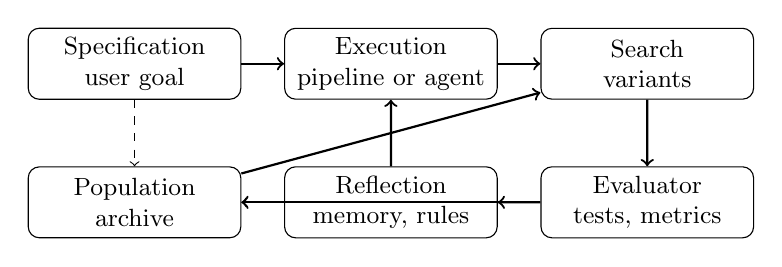
\begin{tikzpicture}[scale=0.88, every node/.style={font=\small}]
  \node[draw, rectangle, rounded corners, align=center, minimum width=2.7cm, minimum height=0.9cm] (spec) at (0,0) {Specification\\user goal};
  \node[draw, rectangle, rounded corners, align=center, minimum width=2.7cm, minimum height=0.9cm] (exec) at (3.7,0) {Execution\\pipeline or agent};
  \node[draw, rectangle, rounded corners, align=center, minimum width=2.7cm, minimum height=0.9cm] (search) at (7.4,0) {Search\\variants};
  \node[draw, rectangle, rounded corners, align=center, minimum width=2.7cm, minimum height=0.9cm] (eval) at (7.4,-2.0) {Evaluator\\tests, metrics};
  \node[draw, rectangle, rounded corners, align=center, minimum width=2.7cm, minimum height=0.9cm] (reflect) at (3.7,-2.0) {Reflection\\memory, rules};
  \node[draw, rectangle, rounded corners, align=center, minimum width=2.7cm, minimum height=0.9cm] (pop) at (0,-2.0) {Population\\archive};
  \draw[->, thick] (spec) -- (exec);
  \draw[->, thick] (exec) -- (search);
  \draw[->, thick] (search) -- (eval);
  \draw[->, thick] (eval) -- (reflect);
  \draw[->, thick] (reflect) -- (exec);
  \draw[->, thick] (eval) -- (pop);
  \draw[->, thick] (pop) -- (search);
  \draw[->, dashed] (reflect) -- (pop);
  \draw[->, dashed] (spec) -- (pop);
\end{tikzpicture}
\caption{Cross-loop composition.  Specification creates executable artifacts; search varies them; evaluators score them; reflection stores lessons; population archives preserve alternatives.}
\label{fig:cross-loop-composition}
\end{figure}

Cross-loop composition creates several design tensions.  The first is speed versus certainty.  Reflection and self-critique are cheap but less reliable.  Full benchmark evaluation is reliable but expensive.  Population archives preserve alternatives but increase storage and evaluation cost.  A practical system uses a cascade: cheap reflection for rapid iteration, tests for candidate filtering, benchmarks for selection, and human review for high-impact updates.

The second tension is specialization versus generality.  Search and population loops can create specialized agents that excel in narrow niches.  Specification-to-execution systems often need general-purpose behavior.  If selection always favors average performance, specialized innovations may disappear.  If selection always favors niche performance, the system may fragment.  MAP-Elites and multi-objective selection address this by preserving best-per-niche candidates while maintaining a default generalist.

The third tension is plasticity versus stability.  A highly plastic system changes quickly in response to feedback.  A stable system resists changes that might cause regressions.  Prompt updates are plastic; weight updates are persistent; code updates are structural.  A mature self-evolution platform should make update levels explicit and require stronger evidence for more persistent changes.  For example, a reflection memory might be added after one failure, but a code patch might require tests, and a model-weight update might require a full evaluation suite.

The fourth tension is autonomous improvement versus governance.  Self-evolution suggests autonomy, but real systems need human oversight, policy constraints, and auditability.  Cross-loop systems should expose their state transitions.  A user or reviewer should be able to inspect what candidate was generated, how it was evaluated, why it was selected, what changed, and what rollback is available.  This is especially important when the system modifies code, tools, permissions, or deployment behavior.

The fifth tension is evaluator evolution.  If the system can improve candidates, it may also need to improve evaluators.  But evaluator changes can invalidate score comparisons across time.  A benchmark version change may make older lineages incomparable.  The solution is to version evaluators, store raw traces where possible, re-evaluate elites under new suites, and separate candidate evolution from evaluator governance.  In scientific discovery systems, evaluator correctness may be the limiting factor; in agent systems, evaluator coverage may be the limiting factor.

A useful architecture pattern is the ``evolution ledger.''  The ledger stores every state transition: candidate ID, parent IDs, generator prompt or policy, evaluator version, scores, traces, selected update, memory changes, and deployment status.  This ledger supports reproducibility, safety review, and meta-learning.  It also enables later analysis: which generators produce useful diversity, which evaluators predict deployment success, which memories reduce repeated failures, and which lineages produce robust improvements.

Another pattern is the ``safe baseline freeze.''  Before self-evolution begins, the system records an incumbent baseline and evaluation suite.  Candidate updates are compared against this baseline.  Regressions trigger rollback or niche-specific storage rather than global replacement.  This pattern is important because self-evolution can otherwise create hidden drift.  A system may look improved on recent tasks while losing older capabilities.  Baseline freezing and regression gates make progress relative and auditable.

A third pattern is ``relative-error control.''  Instead of asking only whether a candidate improved a mean score, the system measures where errors changed.  Did the candidate fix previous failures?  Did it introduce new failures?  Are improvements statistically stable across seeds or task variants?  This matters for stochastic LLM and agent systems.  A single lucky run should not drive persistent updates.  Repeated evaluation and uncertainty estimates should influence selection.

Cross-loop systems can be analyzed by the strongest evaluator in the composition and the deepest update they allow.  A system with weak self-critique and prompt-only updates is low risk but limited.  A system with executable tests and code updates is more powerful and riskier.  A system with self-play verification and weight updates can change broad behavior and therefore needs the strongest governance.  This evaluator-update alignment is one of the main design principles of self-evolving AI.

\subsection{Comparison Table}
\label{subsec:taxonomy-comparison-table}

Table~\ref{tab:method-loop-comparison} summarizes representative methods by loop type, trainability, feedback source, and tasks.  The categories are intentionally coarse.  Many systems span several loops, and implementations vary.  The goal is not to force a single label but to show which mechanism is primary.

\begin{table}[t]
\centering
\small
\begin{tabular}{p{2.8cm} p{3.2cm} p{2.0cm} p{3.4cm} p{3.2cm}}
\hline
\textbf{Method} & \textbf{Primary loop type} & \textbf{Trainable?} & \textbf{Feedback source} & \textbf{Representative tasks} \\
\hline
AutoML-GPT & Specification-to-execution; search over ML pipeline choices & Usually no weight update; may call training jobs & Task cards, data cards, model cards, training logs, validation metrics & AutoML planning, preprocessing, model selection, hyperparameter choices \\
AutoML-Agent & Specification-to-execution; evaluator; reflection across stages & Mostly agent/prompt/pipeline updates & Multi-stage validation, dataset metrics, deployment checks, agent critiques & Full-pipeline AutoML, data processing, model building, evaluation, deployment \\
ADAS & Search over agent architectures; evaluator; possible population & Agent code/prompt/workflow trainability; usually no base-model training & Benchmark task performance, execution traces, success rates & Automated design of agentic systems, tool-using agents, task-specialized workflows \\
OPRO & Search loop over textual candidates & No model training required & Scalar scores placed in optimization prompt & Prompt optimization, mathematical optimization, black-box objective tuning \\
EvoPrompting & Search loop over architecture code & Candidate architectures trained/evaluated; LLM not necessarily trained & Task accuracy or benchmark performance of generated architectures & Code-level NAS, graph neural architectures, reasoning tasks \\
OpenEvolve & Search and evaluator loop over code artifacts & Code evolves; base model often fixed & Tests, benchmarks, execution results, performance metrics & Repository optimization, algorithm improvement, code repair \\
AlphaEvolve & Search + population + evaluator & Code/archive evolves; model may be fixed & Executable evaluators, benchmark scores, archive comparisons & Algorithm discovery, code optimization, scientific or engineering programs \\
FunSearch & Evaluator-driven program search with evolutionary archive & Program population evolves; base LLM fixed & Program execution and objective score & Mathematical discovery, combinatorial constructions, scientific programs \\
Self-Debug & Evaluator + reflection for code repair & No necessary weight update; output/code revised & Execution errors, tests, examples, natural-language debugging feedback & Program synthesis, bug fixing, code explanation and repair \\
CodeEvolve & Evaluator-guided code evolution & Code evolves; possible prompt/memory updates & Unit tests, integration tests, benchmark metrics, traces & Software repair, performance optimization, generated code improvement \\
SelfEvolve & General self-improvement loop; evaluator + reflection/search & Varies: prompt, memory, code, or weights & Task feedback, benchmark scores, validators, self-generated data & Agent improvement, reasoning, code, tool use, benchmark adaptation \\
Reflexion & Reflection loop grounded in evaluator feedback & Memory update; no weight update required & Environment reward, task success/failure, verbal reflections & Agent tasks, reasoning, decision making, code generation \\
Self-Refine & Inference-time reflection/revision & No weight update & LLM-generated critique or feedback prompts & Text generation, reasoning, code, dialogue, style refinement \\
STaR & Reflection to rationale data; training loop & Yes, can fine-tune on rationales & Correct answers, generated rationales, filtering & Reasoning tasks, chain-of-thought improvement, rationale bootstrapping \\
Agent Symbolic Learning & Reflection and search over symbolic agent components & Updates prompts/rules/modules, not necessarily weights & Textual feedback, task loss, component-level critiques & Multi-agent systems, prompt modules, agent architecture improvement \\
LLaMEA & Population loop over meta-heuristic algorithms & Algorithm population evolves & Benchmark optimization performance & Automatic design of meta-heuristics and optimizers \\
DGM & Population + search + evaluator with code self-modification & Agent code evolves; possible archive growth & Benchmarks, task success, code execution, lineage performance & Self-modifying coding agents, open-ended agent improvement \\
SPIN & Self-play/training loop with population-like generated behavior & Yes, model fine-tuning & Self-play comparisons, generated responses, training objectives & Language-model improvement, preference-like self-play, reasoning behavior \\
Absolute Zero & Self-play, self-generated tasks, evaluator, training & Yes, policy/model updates & Verifiable self-generated tasks, code execution or task validators & Zero-data reasoning/code improvement, curriculum generation, RL-style self-improvement \\
\hline
\end{tabular}
\caption{Representative methods mapped to loop type, trainability, feedback source, and task domain.  Several methods compose multiple loops; the table lists the dominant interpretation for taxonomy purposes.}
\label{tab:method-loop-comparison}
\end{table}

The table reveals several trends.  First, early and lightweight methods operate at prompt or output level.  Self-Refine and Reflexion require no model training and can be applied to many tasks, but their updates are limited to current outputs or memory.  Second, code and program-search methods gain power from executable evaluation.  FunSearch, Self-Debug, CodeEvolve, OpenEvolve, and AlphaEvolve can use tests or objective functions, making their feedback more reliable than self-critique alone.  Third, agent-design methods move the unit of evolution from answers to workflows.  ADAS and AutoML-Agent show that roles, tools, and control flow can be searched or revised.  Fourth, population and training methods increase persistence.  DGM and LLaMEA maintain archives; SPIN and Absolute Zero can update weights or policies.

The comparison also shows why ``trainable'' is not a binary property.  A system can train a candidate model while keeping the LLM generator fixed.  AutoML-GPT may train ML models as part of generated pipelines but does not necessarily train the planner.  EvoPrompting may evaluate trained architectures while the language model remains unchanged.  STaR and SPIN update model weights.  Reflexion updates memory.  DGM updates code.  Population methods update archives.  A survey of self-evolution should therefore specify the update substrate rather than simply asking whether the method trains.

Feedback sources form a hierarchy.  Self-feedback is cheap but weak.  Human feedback is meaningful but expensive and variable.  Benchmark feedback is repeatable but can be overfit.  Execution feedback is strong for code but only covers specified properties.  Deployment feedback is realistic but risky and delayed.  The best systems combine feedback sources.  For example, an agent may use self-critique before running, tests during development, benchmark suites before acceptance, and human review before deployment.

The table also suggests a research gap: many methods optimize candidates but do not provide a complete governance layer.  They may lack evaluator versioning, lineage records, rollback, safety constraints, or cross-task regression.  As self-evolution moves from papers to production systems, these engineering layers become part of the scientific object.  A method that improves a score without reproducible lineage is difficult to trust.  A method that stores improvements without regression checks may degrade silently.  A method that changes code or weights without audit trails is hard to govern.

\subsection{Design Dimensions Across the Five Loops}
\label{subsec:taxonomy-design-dimensions}

Beyond method names, self-evolving systems can be compared along design dimensions.  The first dimension is the \emph{update substrate}: output, prompt, memory, workflow, code, data, archive, or weights.  Output updates are temporary; prompt and memory updates are lightweight; workflow and code updates are structural; data and weight updates are statistical; archive updates are population-level.  The update substrate determines persistence, reversibility, and safety burden.

The second dimension is the \emph{candidate generator}.  It can be a single LLM, a multi-agent planner, an evolutionary operator, a learned controller, a random sampler, a Bayesian optimizer, or a hybrid.  LLM generators are flexible and semantic, but they need strong constraints.  Evolutionary operators are simple and diverse, but may be inefficient without semantic guidance.  Multi-agent generators can decompose tasks, but require coordination and can amplify communication errors.  Hybrid generators are likely to dominate because they can combine structured search with language understanding.

The third dimension is the \emph{fitness signal}.  Fitness can be direct or proxy, dense or sparse, deterministic or noisy, scalar or structured.  A direct deterministic evaluator, such as a compiler or exact checker, supports aggressive search.  A noisy proxy evaluator, such as an LLM judge, requires caution and repeated validation.  Sparse rewards make reflection and curriculum generation valuable.  Structured traces make repair easier.  Multi-objective fitness is often necessary because real artifacts must trade off task success, cost, latency, robustness, and safety.

The fourth dimension is \emph{memory}.  Some systems have no memory beyond the current prompt.  Others store examples, reflections, logs, lineages, or learned parameters.  Memory can be episodic, semantic, procedural, or archival.  Episodic memory stores traces of attempts.  Semantic memory stores generalized lessons.  Procedural memory stores updated prompts, rules, or code.  Archival memory stores candidate populations and their metadata.  Weight memory stores experience in parameters.  Each memory type has different retrieval and forgetting problems.

The fifth dimension is \emph{selection pressure}.  Greedy selection maximizes immediate score.  Conservative selection requires improvement beyond uncertainty.  Diversity-preserving selection maintains niches.  Risk-aware selection penalizes safety violations and regressions.  Human-gated selection requires approval for certain updates.  Curriculum selection chooses tasks that maximize learning.  The selection policy shapes the system's long-term trajectory.

The sixth dimension is \emph{autonomy}.  Some loops are human-in-the-loop: users approve plans, edits, or deployments.  Others are autonomous within a sandbox.  Others are fully automated training loops.  Autonomy should increase only with evaluator reliability and rollback capability.  A system may autonomously revise a draft but require review for code changes, and require stricter governance for model-weight updates.

The seventh dimension is \emph{openness}.  A closed-loop system optimizes a fixed task set.  An open-ended system can generate new tasks, new descriptors, new evaluators, or new goals.  Open-endedness is attractive because it can discover unexpected capabilities, but it is difficult to evaluate.  Absolute Zero-style self-generated tasks and DGM-style open-ended archives point in this direction.  The challenge is to prevent drift into trivial, unsafe, or ungrounded objectives.

The eighth dimension is \emph{lineage visibility}.  In a self-evolving system, knowing that a candidate is good is not enough; we want to know where it came from.  Lineage reveals which parent candidates, prompts, memories, or code changes produced an improvement.  It supports reproducibility and debugging.  It also enables meta-learning: the system can learn which mutation prompts or design patterns historically worked.

These dimensions help interpret methods that do not fit neatly into one loop.  For example, a system may use Reflexion-style memory inside an ADAS search.  Its primary loop might be search, but its memory dimension is reflection.  A system may use MAP-Elites for code candidates and STaR-style rationale training for a generator.  Its population and training dimensions are both important.  The five-loop taxonomy is therefore a first layer; design dimensions provide a second layer.

\subsection{Implications for Future Self-Evolving AI Systems}
\label{subsec:taxonomy-implications}

The five-loop taxonomy suggests several principles for building future systems.  First, every self-evolving system should explicitly declare its evolvable substrate.  Users and reviewers should know whether the system is allowed to change outputs, prompts, memories, workflows, code, data, archives, or weights.  Hidden update channels make governance impossible.  A system that claims to be a simple assistant but silently changes its own tool policies is riskier than one that openly maintains a versioned agent configuration.

Second, evaluator strength should match update depth.  Prompt-level revisions can be guided by self-critique and lightweight tests.  Memory updates need evidence and retrieval scope.  Code updates need executable tests and rollback.  Workflow updates need integration evaluation.  Weight updates need broad benchmarks and safety audits.  Population archive updates need metadata and quarantine status.  This principle prevents a common failure: using weak feedback to justify strong updates.

Third, systems should preserve baselines and lineages.  Self-evolution should not erase the path of improvement.  Baselines make regressions visible.  Lineages make improvements explainable.  Archives make diversity recoverable.  A candidate that is not selected globally may still be valuable later as a parent or niche specialist.  This is why population methods and evolution ledgers are likely to become infrastructure rather than optional research details.

Fourth, reflection should be grounded and scoped.  Natural-language memory is powerful because it is cheap and interpretable, but it can become harmful if unverified.  Reflections should cite the feedback that produced them, indicate the component or domain to which they apply, and be revisable.  Systems should measure whether memories improve future outcomes.  Memory should be treated as a hypothesis store, not an unquestioned truth store.

Fifth, search spaces should be designed, not merely opened.  LLMs can edit almost anything, but unrestricted edit spaces are inefficient and unsafe.  Good self-evolution systems define interfaces, templates, schemas, and constraints that make useful variation likely.  AutoML systems use pipeline components; ADAS uses agent-design grammars or program templates; code-evolution systems use tests and patch boundaries; MAP-Elites uses descriptors.  Structure helps the generator explore without producing invalid artifacts.

Sixth, self-evolution should include negative results.  Failed candidates, rejected patches, broken prompts, and harmful memories are valuable data.  They teach the generator what not to do, help evaluators identify blind spots, and prevent repeated mistakes.  A system that stores only successes loses much of the evolutionary signal.  However, negative results must be compressed and indexed so they do not overwhelm context.

Seventh, deployment should be separated from discovery.  Population archives may contain experimental candidates that are useful for search but unsafe for users.  The system should distinguish between discovered, validated, approved, and deployed states.  A candidate can be a research elite without being production-ready.  This distinction allows open-ended exploration while maintaining operational safety.

Eighth, cross-loop composition should be observable.  When a system improves, observers should be able to tell whether the improvement came from better specification parsing, broader search, stronger evaluation, reflection memory, population diversity, or weight training.  Without this decomposition, results are hard to reproduce and compare.  The five-loop taxonomy provides a reporting template: describe the state, generator, evaluator, selector, update, and loop composition.

Finally, the field needs benchmarks that evaluate evolution rather than static performance.  Traditional benchmarks ask how well a fixed model performs.  Self-evolution benchmarks should ask how quickly and safely a system improves over a sequence of tasks, how well it preserves prior capabilities, how efficiently it uses evaluation budget, how robustly it generalizes, and how transparent its updates are.  Metrics should include improvement curves, regression rates, archive diversity, update validity, cost, and human auditability.


\subsection{Failure Modes, Safeguards, and Governance Across Loops}
\label{subsec:taxonomy-failure-governance}

A taxonomy of self-evolution is incomplete without a taxonomy of failure.  Every loop creates a characteristic risk because every loop creates a way for the system to change.  The specification-to-execution loop can misunderstand the user's intent and faithfully optimize the wrong objective.  The search loop can exploit quirks of the search space and produce brittle artifacts.  The evaluator loop can reward shortcuts, leak test information, or miss important constraints.  The reflection loop can store false lessons.  The population loop can preserve unsafe variants or amplify a narrow selection pressure.  These failures are not peripheral engineering details; they determine whether self-evolution produces durable improvement or uncontrolled drift.

The first major failure mode is \emph{specification drift}.  A user supplies an initial goal, but the system converts it into an internal task card that omits, distorts, or over-interprets part of the goal.  Once this internal representation becomes the target of search, later iterations may optimize the wrong problem with increasing confidence.  For example, an AutoML agent may treat accuracy as the only metric even though the user cares about calibration and interpretability.  A coding agent may optimize benchmark runtime while ignoring maintainability.  A research agent may maximize the number of collected sources rather than the quality of analysis.  Specification drift is dangerous because all downstream loops can appear to work: candidates improve, evaluators report progress, and reflections become more detailed, but the system is moving in the wrong direction.

Safeguards against specification drift include explicit task cards, assumption logs, human confirmation for ambiguous objectives, and metric pluralism.  A task card should identify the objective, non-objectives, constraints, evaluation criteria, data assumptions, and deployment context.  The system should record which assumptions were inferred rather than provided.  When evaluator results are reported, they should be tied back to the original goal rather than only to internal metrics.  In self-evolving systems, the task card itself may be updated, but such updates should be versioned and reviewed because changing the target can invalidate previous progress.

The second failure mode is \emph{reward hacking}.  A candidate may improve the measured fitness while violating the intended purpose.  In program evolution, a candidate might exploit a test harness, hard-code answers, skip work, or rely on undefined behavior.  In prompt optimization, a candidate may learn phrases that please an LLM judge without improving correctness.  In agent benchmarks, a candidate may exploit environment artifacts or stop early to avoid penalties.  Reward hacking is not unique to self-evolution, but self-evolution intensifies it because repeated search increases the chance of finding evaluator loopholes.

Safeguards against reward hacking include hidden tests, adversarial evaluation, randomized tasks, differential testing, invariant checks, and evaluator ensembles.  For code, tests should include fixed examples, generated cases, and property-based checks.  For agents, tasks should include varied scenarios and anti-cheating monitors.  For LLM judges, outputs should be sampled across paraphrases and judged by multiple criteria.  For AutoML, leakage checks and data-split validation are essential.  The evaluator loop should treat suspiciously large improvements as signals for additional scrutiny rather than automatic success.

The third failure mode is \emph{memory contamination}.  Reflection loops can store inaccurate or overgeneralized lessons.  A memory such as ``always use a tree-based model'' may help one tabular dataset and harm another.  A reflection such as ``the evaluator prefers concise answers'' may be a local artifact rather than a general rule.  A debugging lesson may become obsolete after the codebase changes.  If contaminated memory is retrieved often, it can bias generation and selection across many future tasks.  This turns a single mistaken reflection into a persistent system-level error.

Memory safeguards include evidence-linked reflections, scoped retrieval, confidence scores, expiration, contradiction checks, and performance-based memory validation.  A memory entry should include the task context, evaluator evidence, component affected, and scope.  Retrieval should prefer memories from similar tasks and avoid flooding the prompt with weakly related lessons.  Memories should be revisable when new evidence contradicts them.  The system can also run ablations: compare performance with and without a memory to estimate whether it actually helps.  Treating memory as a hypothesis store rather than a fact store is a central governance principle.

The fourth failure mode is \emph{population bloat}.  Population systems can accumulate too many candidates, many of which are invalid, redundant, unsafe, or poorly documented.  A large archive is not automatically valuable.  Without descriptors, lineage, and selection discipline, it becomes a storage burden.  Worse, an unsafe or low-quality candidate may later be selected as a parent because its metadata is incomplete.  Population bloat also increases evaluation cost: re-testing all candidates under new benchmarks may become infeasible.

Population safeguards include archive schemas, descriptor-based indexing, quarantine states, pruning policies, and re-evaluation schedules.  Each candidate should have parent IDs, mutation summaries, evaluator versions, scores, validity status, safety status, and intended niche.  Candidates that fail safety checks should be stored separately or deleted, not mixed with deployable elites.  Redundant candidates can be merged or pruned.  Archive coverage should be measured, but coverage should not be confused with quality.  A small, well-indexed archive can be more useful than a large unstructured one.

The fifth failure mode is \emph{regression masking}.  A candidate improves on the current target but silently worsens old capabilities.  This is common when selection uses a narrow score.  A prompt optimized for one benchmark may lose generality.  A code optimization may break rare edge cases.  An AutoML pipeline may improve validation accuracy but degrade fairness.  A model fine-tuned through self-play may become overconfident or less helpful outside the training distribution.  Regression masking is dangerous because the system may report improvement honestly according to its current evaluator while still becoming worse in broader terms.

Regression safeguards include frozen baselines, canary tasks, multi-objective scorecards, statistical repeated runs, and rollback.  Before accepting persistent updates, the system should compare candidates against the incumbent on both target tasks and representative prior tasks.  It should track not only mean score but variance, worst-case performance, and failure categories.  If a candidate improves one niche but regresses another, population storage may be preferable to replacement.  The update should be conditional: deploy the candidate only for the niche where it is proven better.

The sixth failure mode is \emph{evaluator drift}.  Evaluators are themselves artifacts: tests change, benchmarks are updated, LLM judges are replaced, metrics are reweighted, and deployment environments evolve.  If evaluator versions are not recorded, historical scores become incomparable.  A candidate may appear to improve because the evaluator became easier.  A population archive may preserve elites selected under obsolete criteria.  Reflection memories may cite feedback from an evaluator that no longer exists.

Evaluator safeguards include versioning, raw trace storage, re-evaluation of elites, and clear separation between evaluator development and candidate selection.  When an evaluator changes, the system should mark old scores as belonging to an older regime.  Important elites should be re-run under the new evaluator.  If raw traces are stored, some metrics can be recomputed without re-running expensive tasks.  Evaluator updates should themselves be reviewed, especially when they alter safety or acceptance criteria.  A self-evolving system should not silently move the goalposts.

The seventh failure mode is \emph{unsafe autonomy escalation}.  A system may begin with low-risk output revision and gradually acquire the ability to modify prompts, tools, code, workflows, or model weights.  Each added update channel increases the possible impact of mistakes.  If governance does not track these channels, the system can become more autonomous than intended.  This is particularly concerning for agents with external tools, network access, file access, or deployment permissions.

Safeguards include capability boundaries, permission tiers, human gates, sandboxing, and deployment separation.  The system should declare which artifacts it may modify and under what conditions.  Code changes should run in isolated environments.  Tool policies should not be self-modified without review.  Weight updates should be separated from online user interaction unless strong controls exist.  Discovery archives should be distinct from production deployments.  The more persistent the update, the more conservative the gate.

The eighth failure mode is \emph{explanation laundering}.  A system may generate plausible explanations for why a candidate improved, even when the actual cause is accidental.  This can happen in reflection loops and in human-facing reports.  If reviewers accept explanations without checking evidence, the system's narrative becomes more trusted than its measurements.  Explanation laundering is a subtle risk because self-evolving systems are often designed to produce logs, reflections, and rationales.  These artifacts are useful, but they are not proof.

Safeguards include evidence-first reporting, links from claims to evaluator outputs, and distinction between measured facts and inferred explanations.  A reflection should say which test failed or which metric changed.  A candidate summary should distinguish ``passed 47/50 tests'' from ``likely improved because of better planning.''  Lineage reports should include actual diffs or structural changes, not only prose.  Human reviewers should be able to audit the evidence trail.

Governance across loops can be summarized by four rules.  First, make the update substrate explicit.  Second, match evaluator strength to update depth.  Third, version every artifact that influences selection.  Fourth, preserve the ability to roll back.  These rules do not prevent all failures, but they make failures observable and recoverable.  Self-evolution without observability is drift; self-evolution with evidence, lineage, and rollback becomes an engineering discipline.

\subsection{Loop Composition Patterns}
\label{subsec:taxonomy-composition-patterns}

The five-loop taxonomy can be used as a design language.  Instead of asking whether a system is self-evolving in the abstract, we can specify a loop composition pattern.  Different applications require different patterns.  A low-risk writing assistant may need only reflection and lightweight evaluation.  A code optimization system needs search, executable evaluation, and rollback.  An AutoML product needs specification-to-execution, search, and evaluator loops.  A research discovery engine needs population archives and strong validators.  A long-term autonomous agent needs all five loops plus governance.

A first pattern is the \emph{reflection-first assistant}.  The system attempts a task, receives feedback, writes a scoped memory, and uses that memory on later attempts.  This pattern is appropriate when tasks repeat, updates should be interpretable, and external evaluation is available but not necessarily executable.  Reflexion-like agents fit here.  The minimal state includes task traces, reflections, and retrieval metadata.  The main risk is memory contamination, so the main safeguard is evidence-linked memory and retrieval scope.

A second pattern is the \emph{test-driven code evolver}.  The system generates code variants, runs tests, stores failures, and accepts only candidates that improve a scorecard without regressions.  Self-Debug, CodeEvolve, OpenEvolve, FunSearch, and AlphaEvolve-like systems occupy this family at different scales.  The main state includes code, tests, benchmark traces, candidate lineage, and an incumbent baseline.  The generator may use LLM-guided mutation and semantic crossover.  The evaluator is decisive: compilers, unit tests, benchmarks, and performance measurements should gate updates.  The main risks are reward hacking, hidden regressions, and unsafe code execution, so sandboxing and regression suites are mandatory.

A third pattern is the \emph{AutoML compiler}.  The system converts user goals into data-processing and model-training pipelines.  It searches over components and hyperparameters, evaluates validation metrics, and reflects on data or modeling failures.  AutoML-GPT and AutoML-Agent illustrate this pattern.  The main state includes task cards, data profiles, pipeline configurations, training logs, and model comparison tables.  The main risks are specification drift, data leakage, and metric overfitting.  Safeguards include explicit assumptions, leakage checks, held-out validation, and human review for deployment.

A fourth pattern is the \emph{agent architecture search engine}.  The system treats agent workflows as candidates.  It varies role definitions, planning strategies, tool access, memory policies, and verification steps.  ADAS and Agent Symbolic Learning are central references.  The state includes agent graphs, prompts, tool schemas, component-level feedback, and benchmark results.  The evaluator must run full tasks, making cost a major constraint.  Cascaded evaluation is useful: cheap static checks, small task suites, then expensive benchmark runs.  The main risks are invalid workflows, coordination failures, and overfitting to benchmark task formats.

A fifth pattern is the \emph{quality-diversity archive}.  The system maintains elites across task niches or behavior descriptors.  MAP-Elites, AlphaEvolve-style archives, DGM, and LLaMEA illustrate this pattern.  It is appropriate when there is no single universally best candidate or when stepping stones matter.  The state includes an archive grid, descriptors, candidate artifacts, parent links, and evaluator versions.  The main benefits are diversity and specialization.  The main risks are population bloat and unsafe archive contents.  Safeguards include descriptors, pruning, quarantine states, and best-per-niche regression checks.

A sixth pattern is the \emph{self-play trainer}.  The system generates tasks, solutions, critiques, or opponent behaviors, verifies them, and uses the resulting data to update model parameters.  SPIN and Absolute Zero-style systems fit here.  This pattern is powerful because it can change the base model rather than only prompts or code.  It is also difficult to govern because weight updates are broad and less interpretable.  The main state includes generated curricula, verification results, training data, model checkpoints, and evaluation suites.  The main risks are degenerate curricula, overfitting, and broad capability regressions.  Safeguards include held-out benchmarks, task diversity metrics, checkpoint comparison, and conservative deployment gates.

These patterns can be layered.  A test-driven code evolver may use a reflection-first assistant to summarize failures.  An AutoML compiler may maintain a quality-diversity archive of pipelines for different data regimes.  An agent architecture search engine may use self-play-generated tasks to expand its benchmark suite.  A self-play trainer may use programmatic evaluators from the code-evolution pattern to verify generated tasks.  The taxonomy encourages such modular composition while keeping responsibilities clear.

A practical design process can begin with five questions.  What artifact should evolve?  What candidates can be generated safely?  What evaluator can be trusted?  What update is allowed without human review?  What history should be retained?  The answers determine the loop composition.  If the artifact is a final response and the evaluator is a user comment, reflection may suffice.  If the artifact is source code and the evaluator is a test suite, search plus evaluator is appropriate.  If the artifact is an agent organization and the evaluator is a task benchmark, architecture search and population archives may be needed.  If the artifact is model weights, training governance is required.

Loop composition also provides a reporting standard for papers.  A self-evolution paper should report the candidate representation, generator prompts or policies, evaluator suite, selection rule, update substrate, memory mechanism, population size or archive policy, compute budget, and regression checks.  Many current papers emphasize final performance but underreport lineage and evaluator details.  As the field matures, reproducibility will require more complete loop descriptions.  Without them, it is hard to know whether a result came from a stronger generator, a larger search budget, a better evaluator, or a favorable benchmark.

The same reporting standard helps product builders.  A self-evolving product should expose user-facing explanations at the right abstraction level.  Users do not need every candidate trace, but they need to know when the system changed, what evidence justified the change, and how to recover if the change is harmful.  Developers need deeper logs: prompts, diffs, tests, scores, and lineage.  Governance teams need policy status, risk flags, evaluator versions, and deployment gates.  The five-loop taxonomy maps naturally to these views.

Finally, loop composition clarifies a central research frontier: meta-evolution.  Once systems can evolve prompts, code, memories, and populations, they can also evolve the generators, evaluators, and selection rules themselves.  LLaMEA already points toward evolving optimizers.  Agent Symbolic Learning points toward updating symbolic components.  Future systems may search over evaluator designs, reflection schemas, archive descriptors, and governance policies.  This is powerful but risky because it changes the rules of evolution.  Meta-evolution should be slower, more audited, and more conservative than ordinary candidate evolution.

\subsection{A Unifying Example: From User Goal to Evolved Agent}
\label{subsec:taxonomy-unifying-example}

Consider a user who asks for an agent that can maintain a small software library.  The user wants the agent to triage issues, write patches, run tests, update documentation, and avoid breaking public APIs.  A non-evolving agent might be hand-designed once and deployed.  A self-evolving system treats the request as the start of a sequence of loops.

The specification-to-execution loop first converts the request into a task card.  The task card states the repository type, allowed files, testing commands, API stability constraints, documentation requirements, and success metrics.  It identifies missing information, such as supported language versions or deployment targets.  It builds an initial agent workflow: issue reader, planner, coder, test runner, reviewer, and documentation updater.  This workflow is executable because each role has prompts, tool permissions, and handoff rules.

The search loop then proposes variants.  One variant adds a static-analysis step before coding.  Another adds a regression-test generator.  Another changes the planning prompt to require API-impact analysis.  Another splits the reviewer into correctness and style reviewers.  Another changes the order of documentation updates.  Each candidate is an agent workflow, not just an answer.  The generator uses prior failures, examples from similar repositories, and constraints from the task card.

The evaluator loop runs candidates on a suite of repository-maintenance tasks.  It measures tests passed, patches applied, API compatibility, documentation completeness, time, and tool-call cost.  It records traces: failed commands, changed files, review comments, and final diffs.  It also includes negative checks, such as whether the agent modified files outside scope or ignored a failing test.  A candidate that solves more issues but frequently changes public APIs is not accepted as a global replacement.

The reflection loop summarizes failures.  If the agent repeatedly forgets to update documentation after changing behavior, a memory is written for the documentation updater.  If the coder frequently breaks public APIs, a reflection is attached to the planning and review components: public interfaces must be inspected before edits and regression tests must include downstream examples.  If a static-analysis tool produces noisy warnings, the memory records when to trust it and when to ignore it.  These memories are scoped to software-maintenance tasks and tied to evaluator evidence.

The population loop preserves specialized workflows.  A low-latency workflow handles simple documentation fixes.  A high-assurance workflow handles API changes.  A dependency-update workflow handles package upgrades.  A bug-fix workflow handles failing tests.  MAP-Elites descriptors might include task type, risk level, latency budget, and required tool depth.  The system does not force one workflow to handle every issue.  Instead, it routes future tasks to the best elite for the niche.

As the system operates, cross-loop interactions become visible.  A new class of issue appears, such as security vulnerability reports.  The specification loop updates the task card schema to include severity and disclosure constraints.  The search loop proposes security-specific reviewers.  The evaluator loop adds vulnerability regression tests.  The reflection loop stores lessons about unsafe patch patterns.  The population loop creates a security-maintenance niche.  If the system later trains a model or adapter on successful traces, the training loop must be evaluated against the frozen baseline to ensure that general coding ability did not regress.

This example shows why self-evolution is not merely ``the model improves itself.''  The model may remain fixed while the system improves dramatically through better specifications, workflows, tests, memories, and archives.  Conversely, a model may be fine-tuned without meaningful self-evolution if there is no closed loop from evaluated experience to targeted update.  The essence is the structured transition from state to candidate to feedback to selected update.

It also shows why safety is inseparable from the taxonomy.  If the agent can edit code, the evaluator must run tests and enforce file boundaries.  If the agent can update its workflow, workflow changes need review.  If it can store memories, memories need scope.  If it can maintain populations, archive candidates need deployment status.  If it can train weights, checkpoints need broad evaluation.  Each loop adds capability and therefore requires a corresponding guardrail.

The same pattern applies beyond software.  In scientific discovery, the specification is a research objective, search proposes hypotheses or programs, evaluators run simulations or proof checks, reflection stores failed hypotheses, and population archives preserve diverse approaches.  In education, the specification is a learning goal, search proposes tutoring strategies, evaluators measure student outcomes, reflection stores pedagogical lessons, and population methods preserve strategies for learner types.  In robotics, the specification is a task, search proposes policies or controllers, evaluators use simulators and real-world tests, reflection stores failure modes, and populations preserve behaviors for environments.  The substrate changes, but the loops remain.


\subsection{Summary}
\label{subsec:taxonomy-summary}

This chapter organized AI self-evolution around five loops.  The specification-to-execution loop turns natural-language goals into executable artifacts, as illustrated by AutoML-GPT, AutoML-Agent, and ADAS.  The search loop explores prompts, architectures, code, workflows, and hyperparameters, as illustrated by OPRO, EvoPrompting, ADAS, OpenEvolve, and AlphaEvolve.  The evaluator loop supplies fitness through tests, benchmarks, validators, execution traces, and deployment metrics, as illustrated by FunSearch, Self-Debug, CodeEvolve, and SelfEvolve.  The reflection loop turns failures into reusable memory and feedback, as illustrated by Reflexion, Self-Refine, STaR, and Agent Symbolic Learning.  The population loop maintains multiple candidates, lineages, and niches, as illustrated by AlphaEvolve, LLaMEA, DGM, SPIN, and Absolute Zero.

The unified formalization $z_{t+1}=u(z_t,g(z_t),e(g(z_t)))$ is intentionally broad.  Its value is that it makes hidden design choices explicit.  What is the state?  What candidates can be generated?  What evaluator is trusted?  How are candidates selected?  What is updated?  How persistent is the update?  How is rollback handled?  These questions cut across AutoML, NAS, program synthesis, agent frameworks, evolutionary computation, and LLM self-improvement.

The main thesis is that self-evolution is a systems property.  It does not arise from generation alone, nor from reflection alone, nor from benchmarking alone.  It arises when generation, evaluation, memory, selection, and update are connected in a persistent loop.  The strength of the system depends on the alignment between evaluator quality and update power.  Weak evaluators can support lightweight revisions; strong executable evaluators can support code and population evolution; broad validated feedback can support training-time updates.

The taxonomy also clarifies why the field is converging.  AutoML contributes executable pipeline construction.  NAS contributes architecture search and benchmark methodology.  Evolutionary computation contributes population, diversity, and selection.  Program synthesis contributes test-driven generation and repair.  Agent research contributes tool use, memory, and multi-agent organization.  LLM self-improvement contributes reflection, synthetic data, and self-play.  The next generation of systems will likely combine all five loops into platforms that can receive specifications, generate artifacts, evaluate them, remember failures, maintain candidate populations, and update themselves under governance.

For survey purposes, the five-loop taxonomy provides a map.  For system builders, it provides a checklist.  A self-evolving AI system should specify its state, candidates, evaluator, selection policy, update substrate, memory, population strategy, and safety gates.  Methods can then be compared not only by final score but by how they evolve, how safely they update, and how much of their improvement is reproducible.  This is the foundation for treating AI self-evolution as a coherent research and engineering discipline rather than a loose collection of prompting tricks, AutoML tools, and agent demos.
